\documentclass{minimal}
\usepackage{graphicx,color}
\usepackage[utf8]{inputenc}
\usepackage[papersize={420.00bp,298.00bp},text={420.00bp,298.00bp}]{geometry}
\begin{document}
\centering
% Title: gl2ps_renderer figure
% Creator: GL2PS 1.4.2, (C) 1999-2020 C. Geuzaine
% For: Octave
% CreationDate: Mon Dec 12 15:30:47 2022
\setlength{\unitlength}{1pt}
\begin{picture}(0,0)
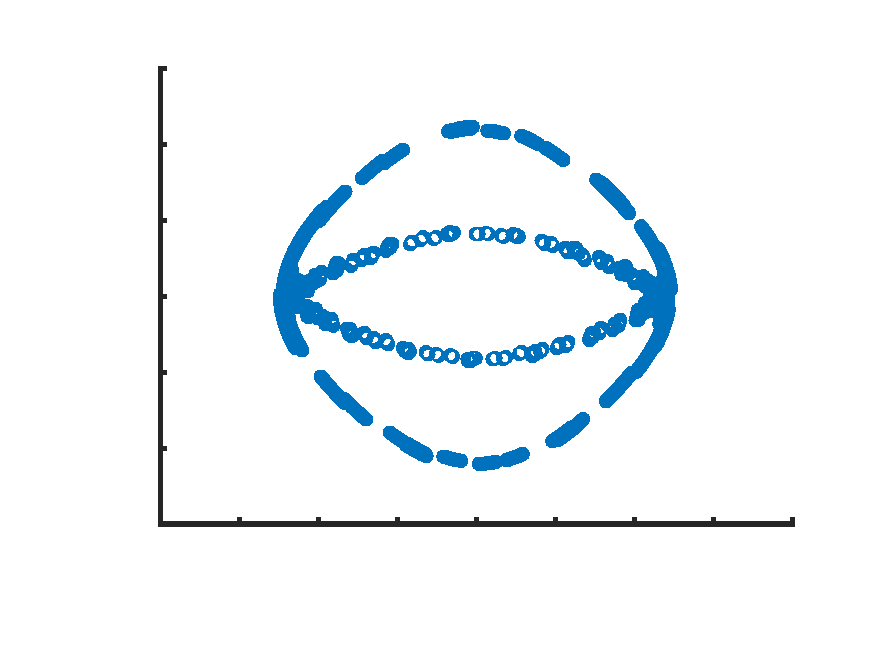
\includegraphics[scale=1]{DoublePoincare-inc}
\end{picture}%
\begin{picture}(420,298)(0,0)
\fontsize{22}{0}\selectfont\put(59.0088,46.3695){\makebox(0,0)[t]{\textcolor[rgb]{0.15,0.15,0.15}{{-0.8}}}}
\fontsize{22}{0}\selectfont\put(112.552,46.3695){\makebox(0,0)[t]{\textcolor[rgb]{0.15,0.15,0.15}{{-0.6}}}}
\fontsize{22}{0}\selectfont\put(166.095,46.3695){\makebox(0,0)[t]{\textcolor[rgb]{0.15,0.15,0.15}{{-0.4}}}}
\fontsize{22}{0}\selectfont\put(219.638,46.3695){\makebox(0,0)[t]{\textcolor[rgb]{0.15,0.15,0.15}{{-0.2}}}}
\fontsize{22}{0}\selectfont\put(273.18,46.3695){\makebox(0,0)[t]{\textcolor[rgb]{0.15,0.15,0.15}{{0}}}}
\fontsize{22}{0}\selectfont\put(326.723,46.3695){\makebox(0,0)[t]{\textcolor[rgb]{0.15,0.15,0.15}{{0.2}}}}
\fontsize{22}{0}\selectfont\put(380.266,46.3695){\makebox(0,0)[t]{\textcolor[rgb]{0.15,0.15,0.15}{{0.4}}}}
\fontsize{22}{0}\selectfont\put(48,62.8793){\makebox(0,0)[r]{\textcolor[rgb]{0.15,0.15,0.15}{{-3}}}}
\fontsize{22}{0}\selectfont\put(48,103.303){\makebox(0,0)[r]{\textcolor[rgb]{0.15,0.15,0.15}{{-2}}}}
\fontsize{22}{0}\selectfont\put(48,143.728){\makebox(0,0)[r]{\textcolor[rgb]{0.15,0.15,0.15}{{-1}}}}
\fontsize{22}{0}\selectfont\put(48,184.152){\makebox(0,0)[r]{\textcolor[rgb]{0.15,0.15,0.15}{{0}}}}
\fontsize{22}{0}\selectfont\put(48,224.576){\makebox(0,0)[r]{\textcolor[rgb]{0.15,0.15,0.15}{{1}}}}
\fontsize{22}{0}\selectfont\put(48,265){\makebox(0,0)[r]{\textcolor[rgb]{0.15,0.15,0.15}{{2}}}}
\fontsize{24}{0}\selectfont\put(219.638,24.3695){\makebox(0,0)[t]{\textcolor[rgb]{0.15,0.15,0.15}{{$\theta_2/(2 \pi)$}}}}
\fontsize{24}{0}\selectfont\put(24,163.94){\rotatebox{90}{\makebox(0,0)[b]{\textcolor[rgb]{0.15,0.15,0.15}{{$\omega_2$}}}}}
\fontsize{24}{0}\selectfont\put(219.638,275){\makebox(0,0)[b]{\textcolor[rgb]{0,0,0}{{Poincaré Section at $\theta_1 = 0$}}}}
\end{picture}
\end{document}
